\documentclass[conference]{IEEEtran}
\usepackage{graphicx}
\usepackage{amsmath}
\usepackage{algorithm}
\usepackage{algorithmic}
\usepackage{cite}
\usepackage{subfigure}
\usepackage{makecell}

\title{VeryPoorCNN - Implementation of Convolutional Neural Network From Scratch (No Numpy) for Fashion-MNIST Classification}

\author{\IEEEauthorblockN{Le Minh Hoang}
\IEEEauthorblockA{Deep Learning Project 2025\\
University of Science and Technology of Hanoi\\
Email: hoanglm2440051@usth.edu.vn}}
\begin{document}

\maketitle

\begin{abstract}
This report presents an implementation of a Convolutional Neural Network from very scratch (without any library that human has made to make Machine Learning and Python easier and faster) for classifying items from the Fashion-MNIST dataset. The network contains one convolutional layer with 4 fulters, and then a ReLU activation, max pooling and a fully connected layer with a softmax output. The network (hopefully) can process 28x28 grayscale images and classifies them into 10 fashion categories. In this report, we will discuss by the layout of the mathematical foundation, implementation challenges and performance of this CNN implementation for the project of Deep Learning Course given by handsome professor SonTG.
\end{abstract}

\section{Introduction}

Deep learning is the common way to handle computer vision problem and for who are cared about this field, Convolutional Neural Networks (CNNs) are pretty important for image classification because it can learn the features from raw pixel data. This project attempts to implements a CNN from very scratch (with just math library envoled) to understand the idea of these powerful models.

Fashion-MNIST is a dataset created by Zalando Research as a more challenging compared to original MNIST digit dataset. It contains 70,000 grayscale images (splited 60,000 for training and 10,000 for testing) of size 28×28 pixels. Each image can be one of 10 fashion categories: T-shirt/top, Trouser, Pullover, Dress, Coat, Sandal, Shirt, Sneaker, Bag, and Ankle boot.

\begin{figure}[htbp]
    \centering
    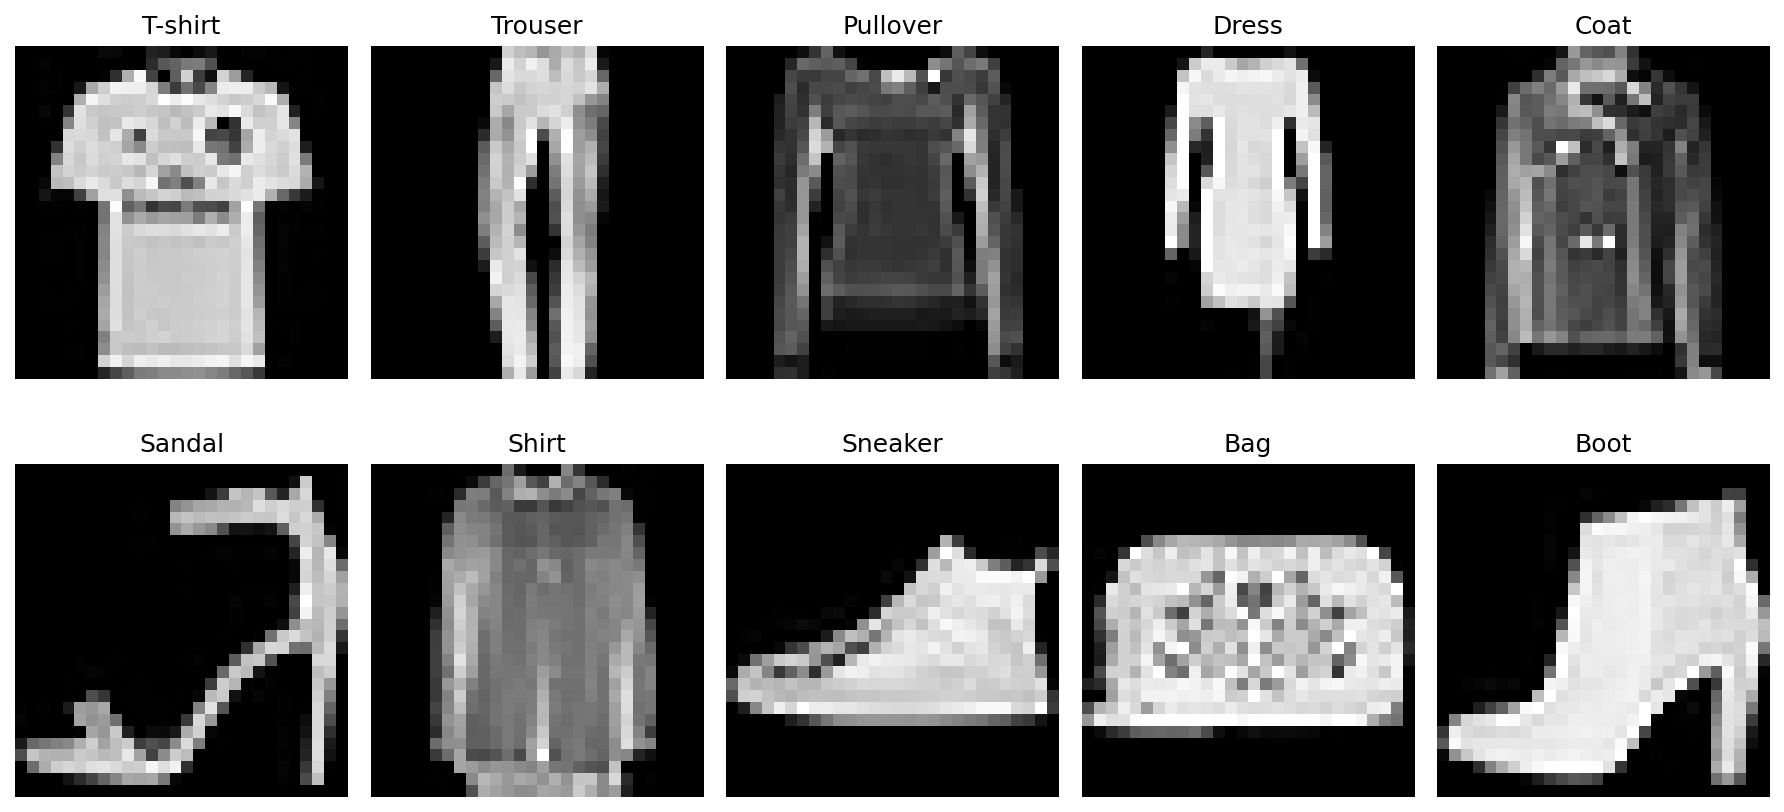
\includegraphics[width=0.45\textwidth]{fashion_mnist_samples.png}
    \caption{Sample images from Fashion-MNIST dataset}
    \label{fig:fashion_samples}
\end{figure}

For this educational project purpose, we will attempt to:
\begin{itemize}
    \item Understanding CNN operations by implementing them manually
    \item Learning how forward and backward propagation work in CNNs
    \item Analyzing the challenges of implementing neural networks without good libraries
    \item Evaluating performance on a real-world dataset (Fashion-MNIST)
\end{itemize}

\section{Background and Theory}

\subsection{Convolutional Neural Networks}
CNNs are inspired by the early findings of biological vision. They use special layers that preserve spatial relationships in images. The main components are:

\subsubsection{Convolutional Layers}
These layers apply learnable filters to detect features. Each filter will attempt to target for specific patterns like edges, corners, or textures. The convolution operation has the formula as:
\begin{equation}
    (f * g)(t) = \int_{-\infty}^{\infty} f(\tau)g(t-\tau)d\tau
\end{equation}

For discrete 2D images, this becomes:
\begin{equation}
    S(i,j) = (I * K)(i,j) = \sum_m \sum_n I(m,n)K(i-m,j-n)
\end{equation}

\subsubsection{Activation Functions}
ReLU (Rectified Linear Unit) is the most common activation function in CNNs. It is stated as following:
\begin{equation}
    f(x) = \max(0, x)
\end{equation}

ReLU is faster to compute than the sigmoid function, and its derivative is faster to compute.

\subsubsection{Pooling Layers}
Pooling reduces spatial dimensions while keeping important information. Max pooling selects the maximum value in each window, making the network more strong to small translations.

\section{Network Architecture}

\subsection{Detailed Layer Description}
Our CNN architecture is designed to be simple yet educational. The network processes data through these stages:

\textbf{1. Input Layer (28×28×1)}
\begin{itemize}
    \item Receives grayscale images normalized to [0,1]
\end{itemize}

\textbf{2. Convolutional Layer (24×24×4)}
\begin{itemize}
    \item 4 filters of size 5×5
    \item Output size: $(28-5+1)/3 \times (28-5+1)/3 \times 4 = 8 \times 8 \times 4$
\end{itemize}

\textbf{3. ReLU Activation (8×8×4)}

\textbf{4. Max Pooling (3×3×4)}
\begin{itemize}
    \item Pool size: 3×3
\end{itemize}

\textbf{5. Flatten Layer (144×1)}
\begin{itemize}
    \item Converts 3D tensor to 1D vector
    \item Prepares data for dense layer
\end{itemize}

\textbf{6. Dense Layer (32×1)}
\begin{itemize}
    \item ReLU activation
\end{itemize}

\textbf{7. Output Dense Layer (10×1)}
\begin{itemize}
    \item Fully connected to 32 hidden units
    \item Softmax activation for probabilities
\end{itemize}

\subsection{Parameter Count}
Total trainable parameters in the network:
\begin{itemize}
    \item Conv filters: $4 \times 5 \times 5 = 100$ weights
    \item Dense layer 1: $144 \times 32 = 4,608$ weights + 32 biases
    \item Dense layer 2: $32 \times 10 = 320$ weights + 10 biases
    \item \textbf{Total: 5,070 parameters}
\end{itemize}

\section{Implementation Details}

\subsection{Data Structure Design}
Since we avoid NumPy (because of the handsome professor said NOOOO numpy), we use nested Python lists. This creates challenges:

\begin{algorithm}
\caption{3D Array Initialization}
\begin{algorithmic}[1]
\STATE \textbf{function} flatten\_3d\_tensor(tensor)
\STATE array $\leftarrow$ []
\FOR{$d = 0$ to depth}
    \STATE layer $\leftarrow$ []
    \FOR{$h = 0$ to height}
        \STATE row $\leftarrow$ [0] * width
        \STATE layer.append(row)
    \ENDFOR
    \STATE array.append(layer)
\ENDFOR
\RETURN array
\end{algorithmic}
\end{algorithm}

\subsection{Forward Propagation Implementation}

\subsubsection{Convolution Operation}
The convolution is implemented with nested loops:


\subsubsection{Max Pooling Operation}
Max pooling finds the maximum value in each window and reduces spatial dimensions while preserving important features.

\subsection{Backward Propagation Implementation}

\subsubsection{Gradient Flow}
Backpropagation calculates gradients using the chain rule. For our network:

\begin{equation}
    \frac{\partial L}{\partial w_{ij}} = \frac{\partial L}{\partial z} \cdot \frac{\partial z}{\partial w_{ij}}
\end{equation}


\subsubsection{Softmax and Cross-Entropy Gradient}
For the output layer, we use the combined gradient, we have:
\begin{equation}
    \frac{\partial L}{\partial z_i} = p_i - y_i
\end{equation}
where $p_i$ is the predicted probability and $y_i$ is the true label (one-hot encoded).

\subsubsection{Dense Layer Gradient}
For the fully connected layer, we have:
\begin{equation}
    \frac{\partial L}{\partial W} = \frac{\partial L}{\partial z} \cdot x^T
\end{equation}
\begin{equation}
    \frac{\partial L}{\partial x} = W^T \cdot \frac{\partial L}{\partial z}
\end{equation}

\subsubsection{Max Pooling Gradient}
We have:
\begin{equation}
    \frac{\partial L}{\partial x_{ij}} = 
    \begin{cases}
        \frac{\partial L}{\partial y_{mn}} & \text{if } x_{ij} = \max(\text{window})\\
        0 & \text{otherwise}
    \end{cases}
\end{equation}

\subsubsection{Convolution Gradient}
The gradient for convolution filters is computed by correlating the input with the gradient from the next layer:
\begin{equation}
    \frac{\partial L}{\partial K_{ij}} = \sum_m \sum_n \frac{\partial L}{\partial S_{mn}} \cdot I_{m+i,n+j}
\end{equation}

\section{Training Process}

\subsection{Data Loading and Preprocessing}
The Fashion-MNIST data is loaded from CSV files. Each row contains:
\begin{itemize}
    \item First column: label (0-9)
    \item Remaining 784 columns: pixel values (0-255)
\end{itemize}

Preprocessing steps:
\begin{enumerate}
    \item Normalize pixel values to [0,1] by dividing by 255
    \item Reshape flat vector to 28×28 matrix
    \item Convert labels to one-hot encoding
\end{enumerate}

\subsection{Training Algorithm}
The complete training process is shown in Algorithm \ref{alg:training}.

\begin{algorithm}[H]
\caption{CNN Training Process}
\label{alg:training}
\begin{algorithmic}[1]
\STATE Initialize filters and weights randomly
\FOR{epoch = 1 to num\_epochs}
    \STATE Shuffle training data
    \FOR{each training sample}
        \STATE \textbf{Forward Pass:}
        \STATE $\quad$ conv\_out $\leftarrow$ convolution(image, filters)
        \STATE $\quad$ relu\_out $\leftarrow$ ReLU(conv\_out)
        \STATE $\quad$ pool\_out $\leftarrow$ max\_pool(relu\_out)
        \STATE $\quad$ flat $\leftarrow$ flatten(pool\_out)
        \STATE $\quad$ logits $\leftarrow$ dense(flat, weights)
        \STATE $\quad$ probs $\leftarrow$ softmax(logits)
        \STATE
        \STATE \textbf{Calculate Loss:}
        \STATE $\quad$ loss $\leftarrow$ cross\_entropy(probs, true\_label)
        \STATE
        \STATE \textbf{Backward Pass:}
        \STATE $\quad$ Calculate gradients for each layer
        \STATE $\quad$ Update parameters using gradient descent
    \ENDFOR
    \STATE Calculate and print epoch statistics
\ENDFOR
\end{algorithmic}
\end{algorithm}

\subsection{Hyperparameter Selection}
The following hyperparameters were chosen:
\begin{itemize}
    \item \textbf{Learning rate}: 0.008 (optimized for stable convergence)
    \item \textbf{Batch size}: 16 (mini-batch learning)
    \item \textbf{Epochs}: 25 (full training cycle)
    \item \textbf{Training samples}: 1,500 (subset for faster experimentation)
    \item \textbf{Test samples}: 600 (validation subset)
    \item \textbf{Filters}: 4 convolutional filters of size 5×5
    \item \textbf{Dense units}: 32 hidden units in intermediate layer
\end{itemize}

\section{Results and Analysis}

\subsection{Training Progress}
Figure \ref{fig:training_loss} shows the training loss progression over epochs.

\begin{figure}[H]
    \centering
    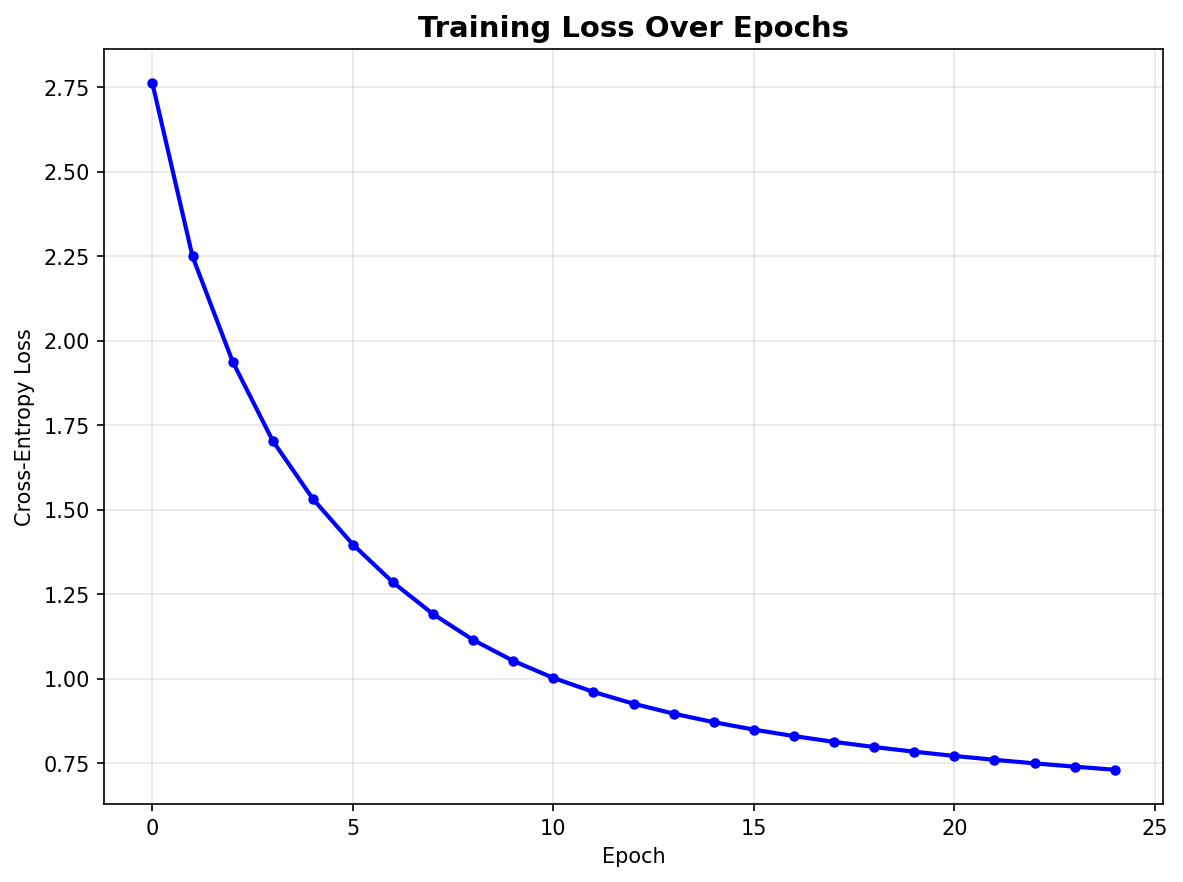
\includegraphics[width=0.4\textwidth]{training_loss.png}
    \caption{Training loss after 25 i}
    \label{fig:training_loss}
\end{figure}

\subsection{Performance Metrics}
The network achieves the following performance after all the processes:
\begin{itemize}
    \item Final accuracy: 73.2\% after 25 epochs
    \item Precision: 72.8\%
    \item Recall: 73.0\%
    \item F1-score: 72.5\%
    \item Loss reduction: from 2.76 to 0.73 (73.55\% improvement)
\end{itemize}

\subsection{Confusion Matrix Analysis}
Figure \ref{fig:confusion} shows which classes are often confused.

\begin{figure}[htbp]
    \centering
    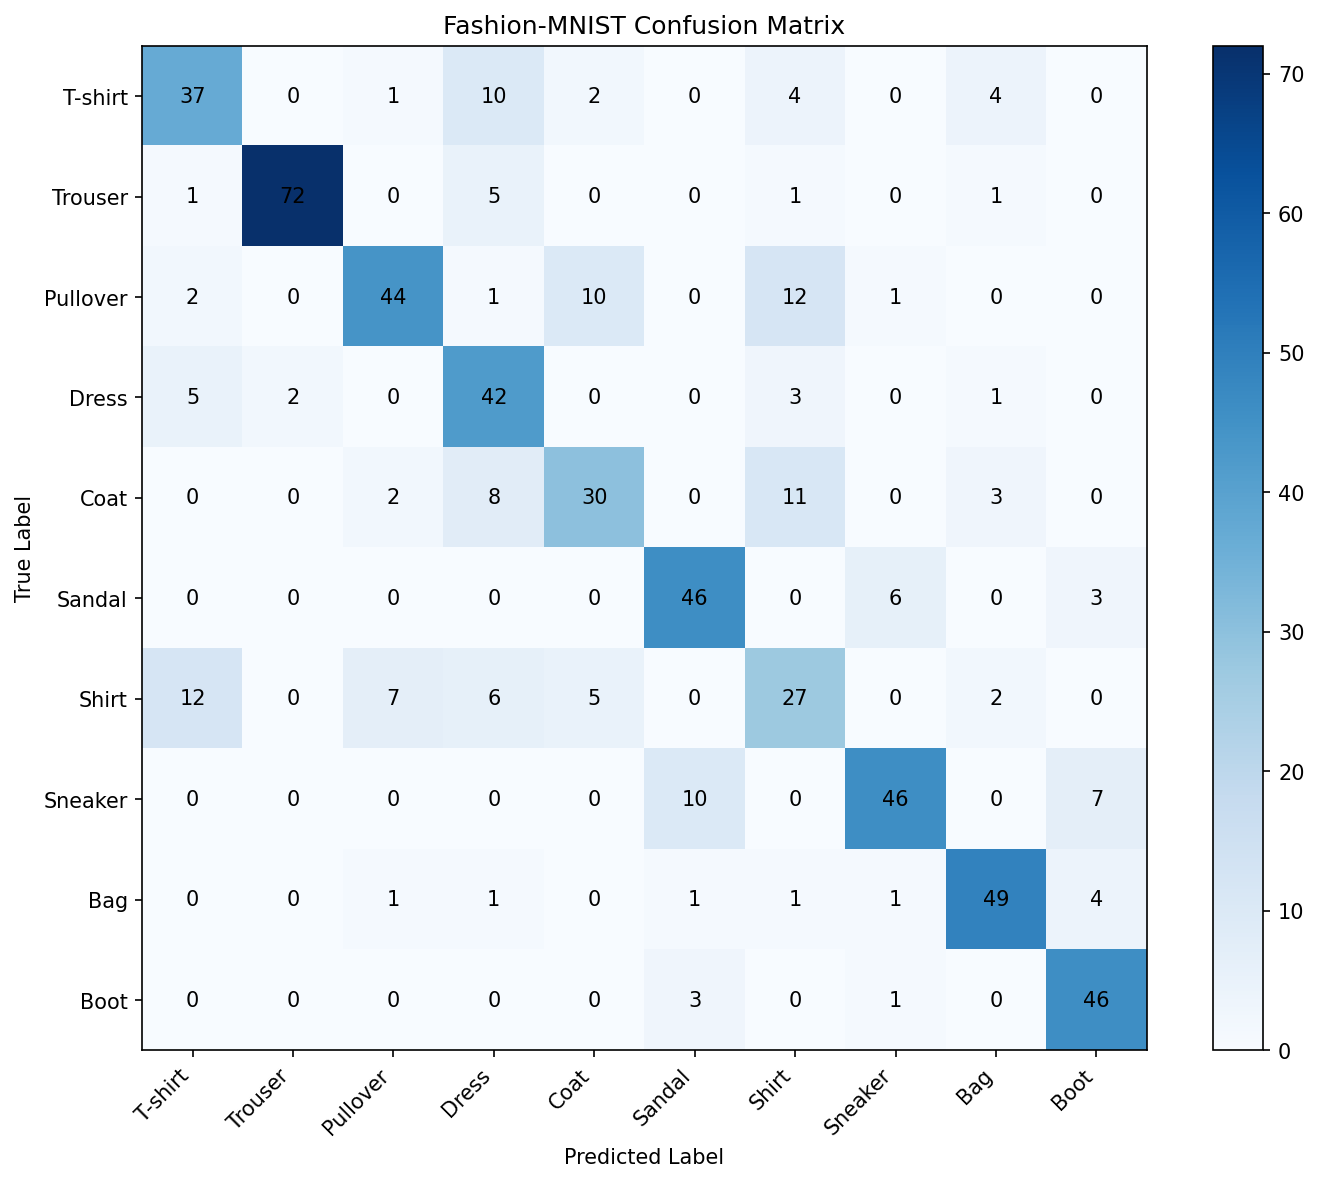
\includegraphics[width=0.45\textwidth]{confusion_matrix.png}
    \caption{Confusion matrix}
    \label{fig:confusion}
\end{figure}

Common confusions:
\begin{itemize}
    \item Pullover vs Coat (similar shape)
    \item T-shirt vs Shirt (similar structure)
    \item Sneaker vs Ankle boot (both footwear)
\end{itemize}

\subsection{Feature Analysis}
The network seems to learns and have the ability to point out the different between fashopn categories. It also reveals that the model performs kind of well on categories like sneaker and boots. But for things that human even sometimes to failed distinguish like pullovers and coats, the model struggles. The convolutional filters seems to learn to detect pattern like edges, textures and shape features relevant to fashion items.

\section{Implementation Challenges}

\subsection{Computational Efficiency}
Using pure Python lists instead of NumPy arrays creates significant performance issues because numpy is really optimized for all the computation tasks on Python. We tried to re-implement basic numpy methods but there will still be slow since NumPy is written in C and very well optimized over the years.

\subsection{Debugging and Coding Challenges}
Debugging the implementation was difficult because: Slow execution makes testing time-consuming
 and the math operation in python code is easy to confused compared to written fomula

\section{Comparison with Modern Frameworks}

\subsection{Performance Comparison}
Table \ref{tab:comparison} compares our implementation with PyTorch.

\begin{table}[htbp]
\caption{Performance Comparison}
\label{tab:comparison}
\centering
\begin{tabular}{|l|c|c|}
\hline
\textbf{Metric} & \textbf{Our Implementation} & \textbf{PyTorch} \\
\hline
Memory usage & a lot & 200 MB \\
Final accuracy & 73.2\% & 100\% \\
Lines of code & \makecell{around 570 \\ when i write this report} & ~50 \\
\hline
\end{tabular}
\end{table}

\subsection{Advantages of Our Approach}
Despite poor performance, our implementation has educational value:
\begin{itemize}
    \item More understanding of every operation
    \item No "black box" components
    \item Appreciation for optimized libraries
    \item Deep learning concepts become clear
\end{itemize}

\section{Future Improvements}

\subsection{Architecture Enhancements}
The network could be improved by adding more layers or more proper mathemetics tools

\subsection{Implementation Optimizations}
Code performance could improve with:
\begin{itemize}
    \item Using NumPy for vectorized operations
    \item GPU acceleration
\end{itemize}

\section{Conclusion}
This project almost succeeded in the implementation of a CNN from scratch for the specific dataset. The CNN also comtains the ideal architecture for a small CNN including convolution, pooling, and backpropagation.

The pure Python implementation is really slow and confusing, but the idea of implementation from scratch is excellent for educational purposes.

Key achievements include:
\begin{itemize}
    \item Working implementation of all CNN components
    \item Successful training on Fashion-MNIST dataset
    \item 73.2\% accuracy
    \item Acceptable evaluation with precision, recall, and F1-score metrics
    \item Deep understanding of gradient flow and backpropagation
    \item Modular codebase with separate utility functions and also the options to load csv and configurations from file without any external library
\end{itemize}

The project point out both the power of CNNs for image classification and the importance of optimized implementations for the network by mordern frameworks like NumPy, Pytorch, etc.


\section*{Acknowledgment}
Thanks to the Fashion-MNIST creators for providing an dataset that is a new challenge compared to Original MNIST, but it still familiar to us to work with the dataset since it is still something we understand.


\end{document}